\documentclass[]{article}
\usepackage{lmodern}
\usepackage{amssymb,amsmath}
\usepackage{ifxetex,ifluatex}
\usepackage{fixltx2e} % provides \textsubscript
\ifnum 0\ifxetex 1\fi\ifluatex 1\fi=0 % if pdftex
  \usepackage[T1]{fontenc}
  \usepackage[utf8]{inputenc}
\else % if luatex or xelatex
  \ifxetex
    \usepackage{mathspec}
  \else
    \usepackage{fontspec}
  \fi
  \defaultfontfeatures{Ligatures=TeX,Scale=MatchLowercase}
\fi
% use upquote if available, for straight quotes in verbatim environments
\IfFileExists{upquote.sty}{\usepackage{upquote}}{}
% use microtype if available
\IfFileExists{microtype.sty}{%
\usepackage{microtype}
\UseMicrotypeSet[protrusion]{basicmath} % disable protrusion for tt fonts
}{}
\usepackage[margin=1in]{geometry}
\usepackage{hyperref}
\hypersetup{unicode=true,
            pdfborder={0 0 0},
            breaklinks=true}
\urlstyle{same}  % don't use monospace font for urls
\usepackage{graphicx,grffile}
\makeatletter
\def\maxwidth{\ifdim\Gin@nat@width>\linewidth\linewidth\else\Gin@nat@width\fi}
\def\maxheight{\ifdim\Gin@nat@height>\textheight\textheight\else\Gin@nat@height\fi}
\makeatother
% Scale images if necessary, so that they will not overflow the page
% margins by default, and it is still possible to overwrite the defaults
% using explicit options in \includegraphics[width, height, ...]{}
\setkeys{Gin}{width=\maxwidth,height=\maxheight,keepaspectratio}
\IfFileExists{parskip.sty}{%
\usepackage{parskip}
}{% else
\setlength{\parindent}{0pt}
\setlength{\parskip}{6pt plus 2pt minus 1pt}
}
\setlength{\emergencystretch}{3em}  % prevent overfull lines
\providecommand{\tightlist}{%
  \setlength{\itemsep}{0pt}\setlength{\parskip}{0pt}}
\setcounter{secnumdepth}{0}
% Redefines (sub)paragraphs to behave more like sections
\ifx\paragraph\undefined\else
\let\oldparagraph\paragraph
\renewcommand{\paragraph}[1]{\oldparagraph{#1}\mbox{}}
\fi
\ifx\subparagraph\undefined\else
\let\oldsubparagraph\subparagraph
\renewcommand{\subparagraph}[1]{\oldsubparagraph{#1}\mbox{}}
\fi

%%% Use protect on footnotes to avoid problems with footnotes in titles
\let\rmarkdownfootnote\footnote%
\def\footnote{\protect\rmarkdownfootnote}

%%% Change title format to be more compact
\usepackage{titling}

% Create subtitle command for use in maketitle
\newcommand{\subtitle}[1]{
  \posttitle{
    \begin{center}\large#1\end{center}
    }
}

\setlength{\droptitle}{-2em}

  \title{}
    \pretitle{\vspace{\droptitle}}
  \posttitle{}
    \author{}
    \preauthor{}\postauthor{}
    \date{}
    \predate{}\postdate{}
  

\begin{document}

\section{\texorpdfstring{\textbf{What made you happy
today?}}{What made you happy today?}}\label{what-made-you-happy-today}

\subsection{\texorpdfstring{\textbf{Does cause of happniess differ
between genders, parenthoods, reflection periods, and
categories?}}{Does cause of happniess differ between genders, parenthoods, reflection periods, and categories?}}\label{does-cause-of-happniess-differ-between-genders-parenthoods-reflection-periods-and-categories}

By Yanzi Shen \newline

 HappyDB is ``a corpus of 100,000 crowd-sourced happy moments''. In this
project, I apply text mining techniques and natural language processing
to derive interesting finds in this collection of happy moments and look
deeper into the causes that make us happy.

\subsection{Word clouds of happy
moments}\label{word-clouds-of-happy-moments}

\subsubsection{Overall causes}\label{overall-causes}

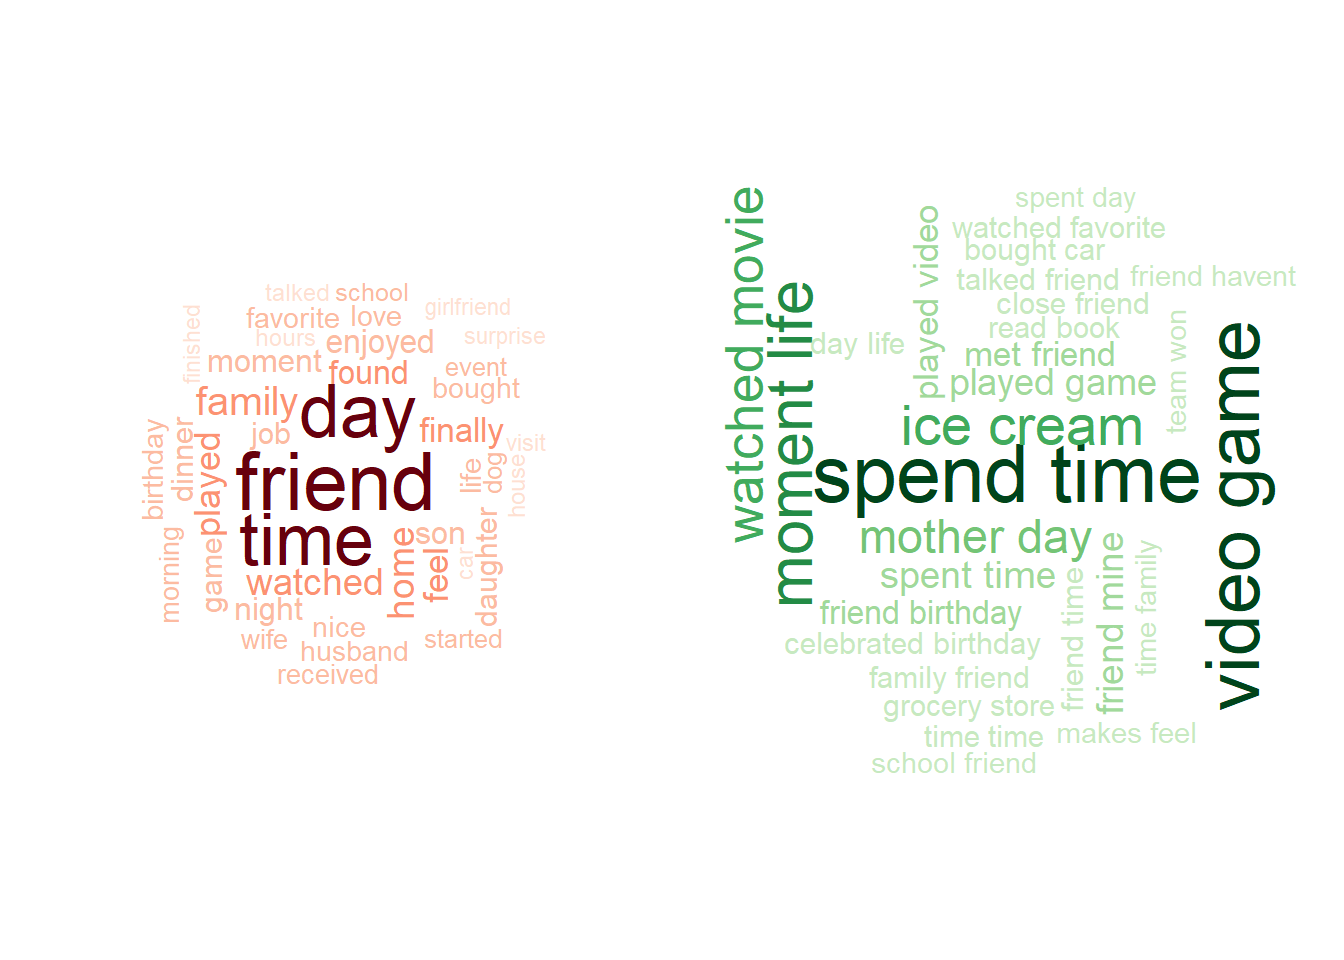
\includegraphics{preview_files/figure-latex/wordcould overall-1.pdf}
First of all, we take a look the most popular words in all happy
moments. The left is the most frequent single words and right is the
most frequent pairs of words. The deeper the word, the more important it
is. We can see that he most frequent single words is ``friend'',
``day'', ``time''. The most frequent pairs of words are ``spend time'',
``video game'', ``moment life''. Those words show the general causes of
happiness.

\subsubsection{Female vs Male}\label{female-vs-male}

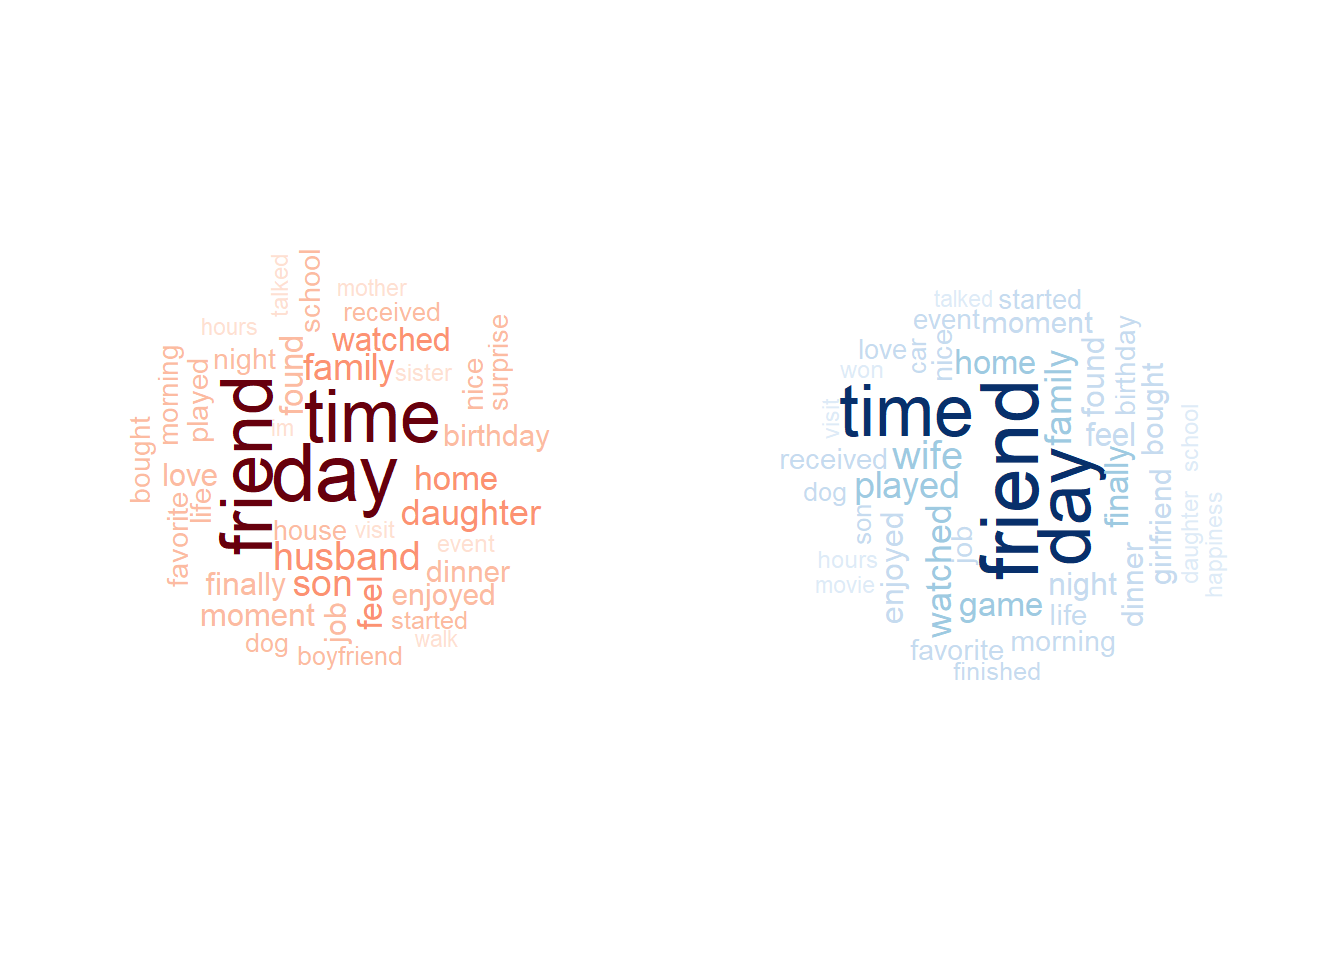
\includegraphics{preview_files/figure-latex/wordcould of single word by gender-1.pdf}
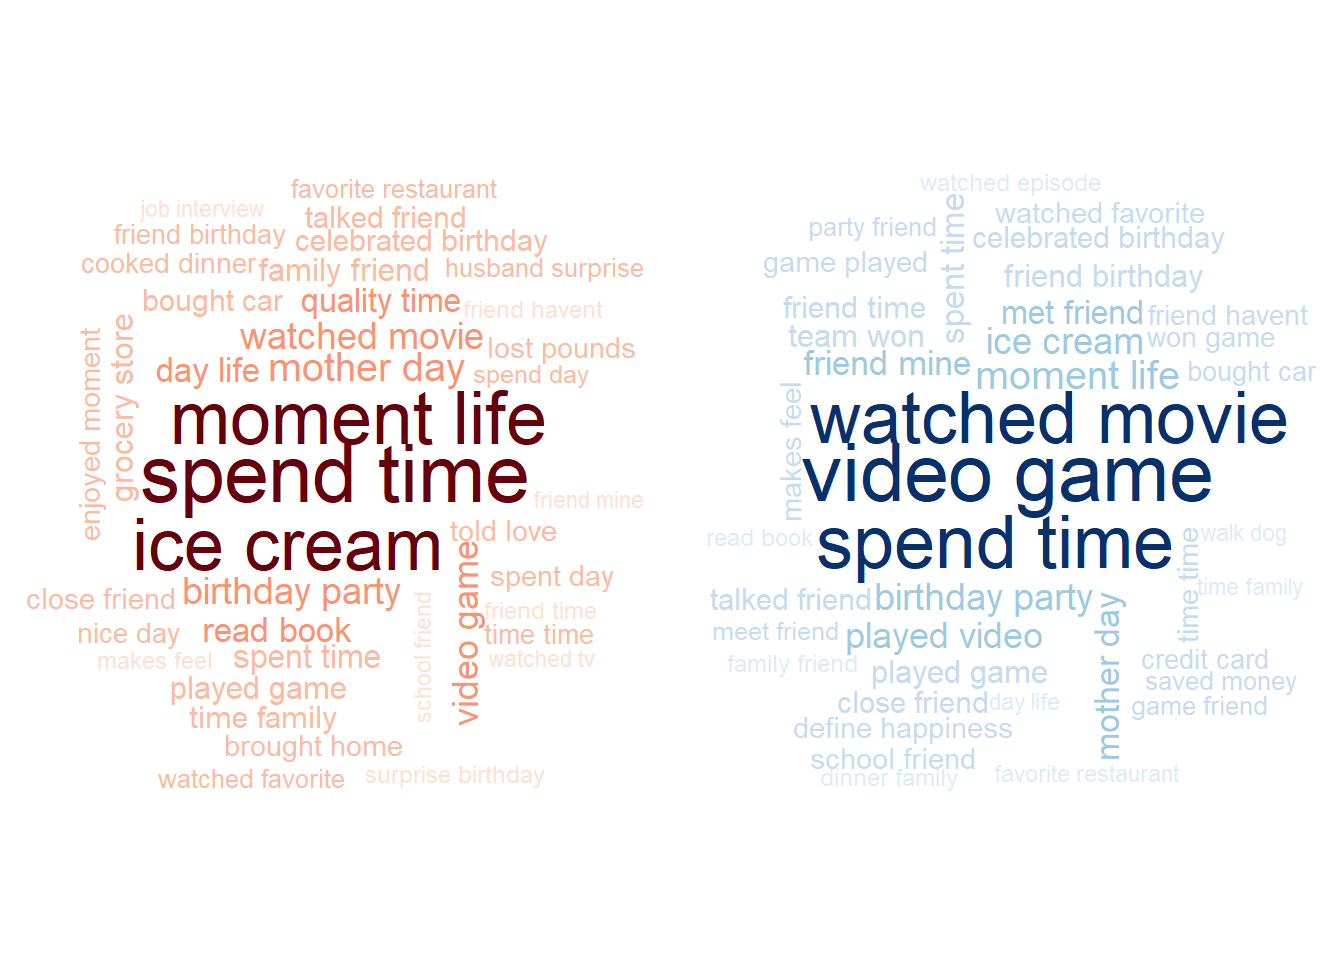
\includegraphics{preview_files/figure-latex/wordcould of pairs of words by gender-1.pdf}
Left is the most frequent causes of happiness in female and right is the
most frequent causes of happiness in male.

There is no difference in the top three single words in gender. However,
if we takes deep look, we can see that more females mention that
``son'', ``daughter'', ``home'' make them happy. And males mention more
about ``played'', ``game''. It seems that woman cares more about family
and males cares more about entertainments.

There are differences in the top three pairs of words. For females, they
are ``moment life'', ``spend time'' and ``ice creams''. For male, they
are ``video game'', ``spend time'', and ``watched movie''. Same as what
shows in single words, entertainment can easily make men happy. It is
interesting to find that ``ice creams'' appears in the top three causes.
Maybe we can say that there are more foodies in female than males. In
addition, ``lose pounds'' appears word cloud of female. It may prove
that females care more about keeping fit than males.

\subsubsection{Parenthood vs Without
Parenthood}\label{parenthood-vs-without-parenthood}

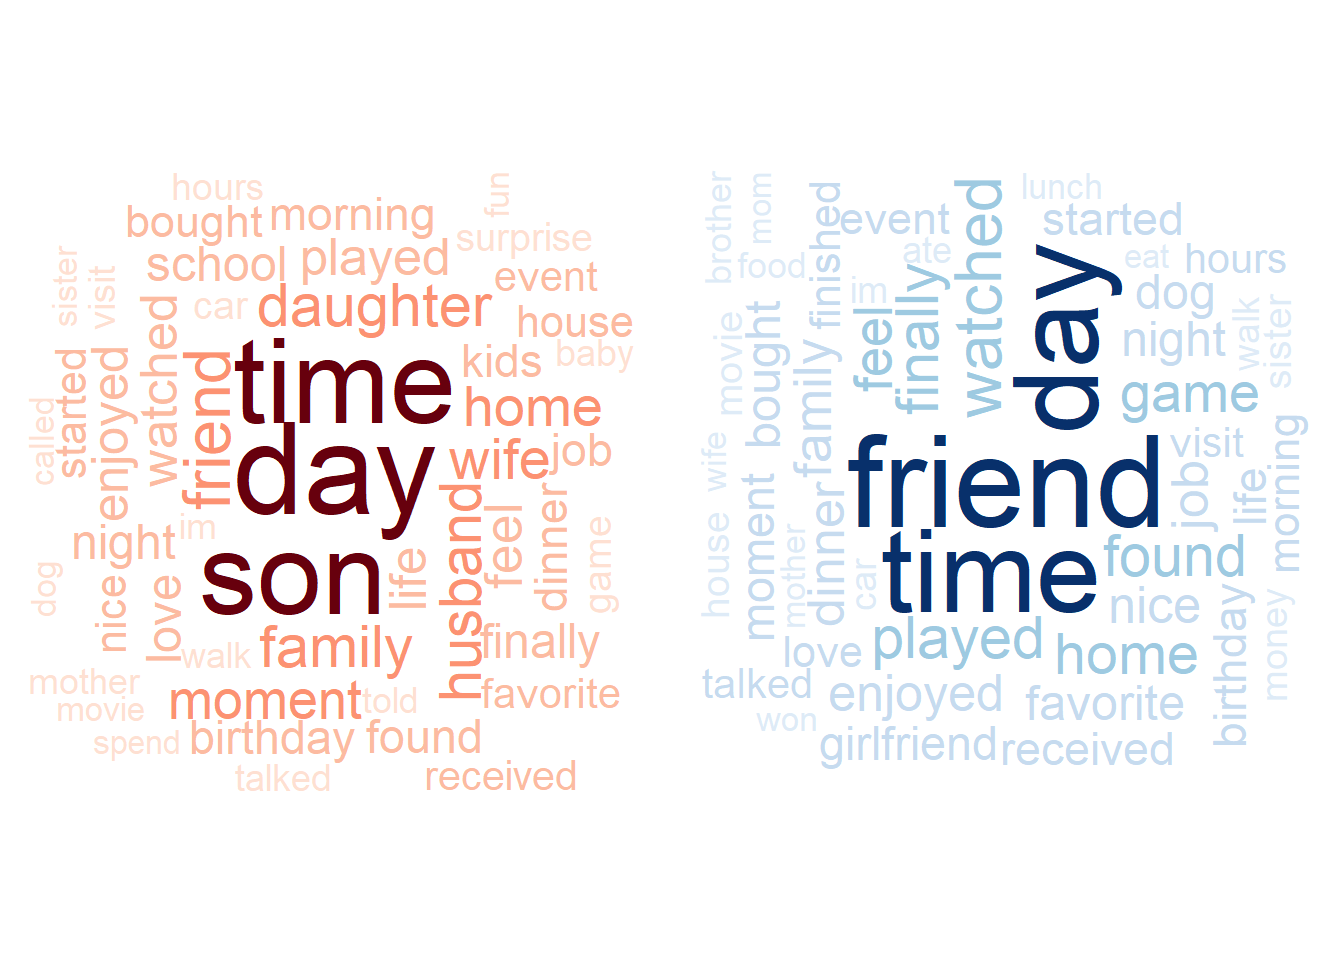
\includegraphics{preview_files/figure-latex/wordcould of single word by parenthood-1.pdf}

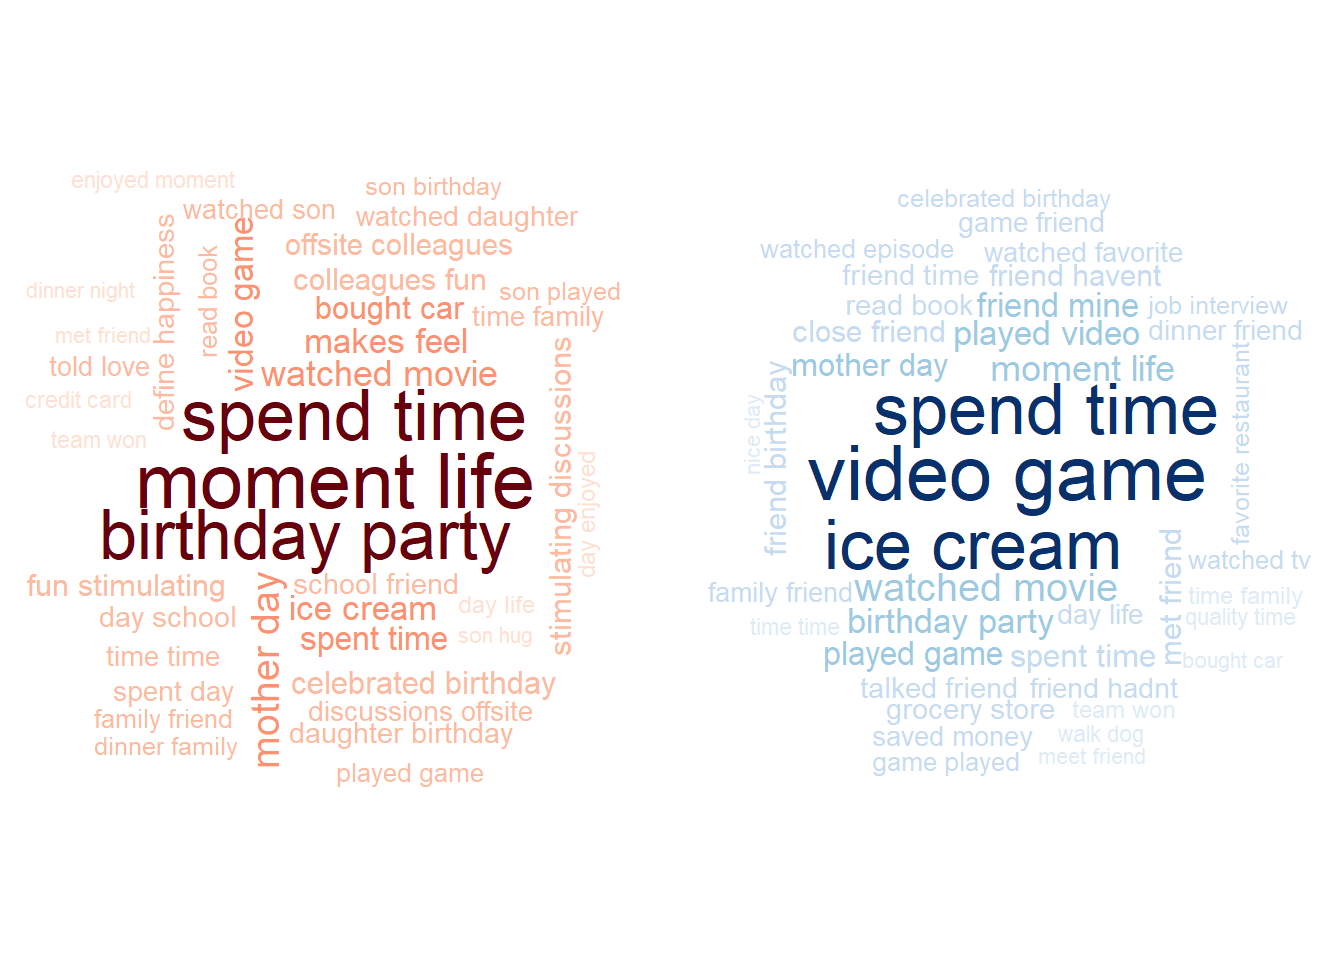
\includegraphics{preview_files/figure-latex/wordcould of pair of words by parenthood-1.pdf}
Left is the most frequent causes of happiness for someone being a parent
and right is the most frequent causes of happiness for someone not being
a parents.

The top frequent single words show that people having children will
easily be happy because of their kid. People not having children are
more likely to be happy because of friends.

In the pairs of words, people having children will easily be happy
because of ceremonies and anniversaries, like ``birthday party'',
``mother day''. People not having children are more likely to be happy
because of food or entertainment, like" ice cream``,''video games``.

\subsubsection{24 hours vs 3 months}\label{hours-vs-3-months}

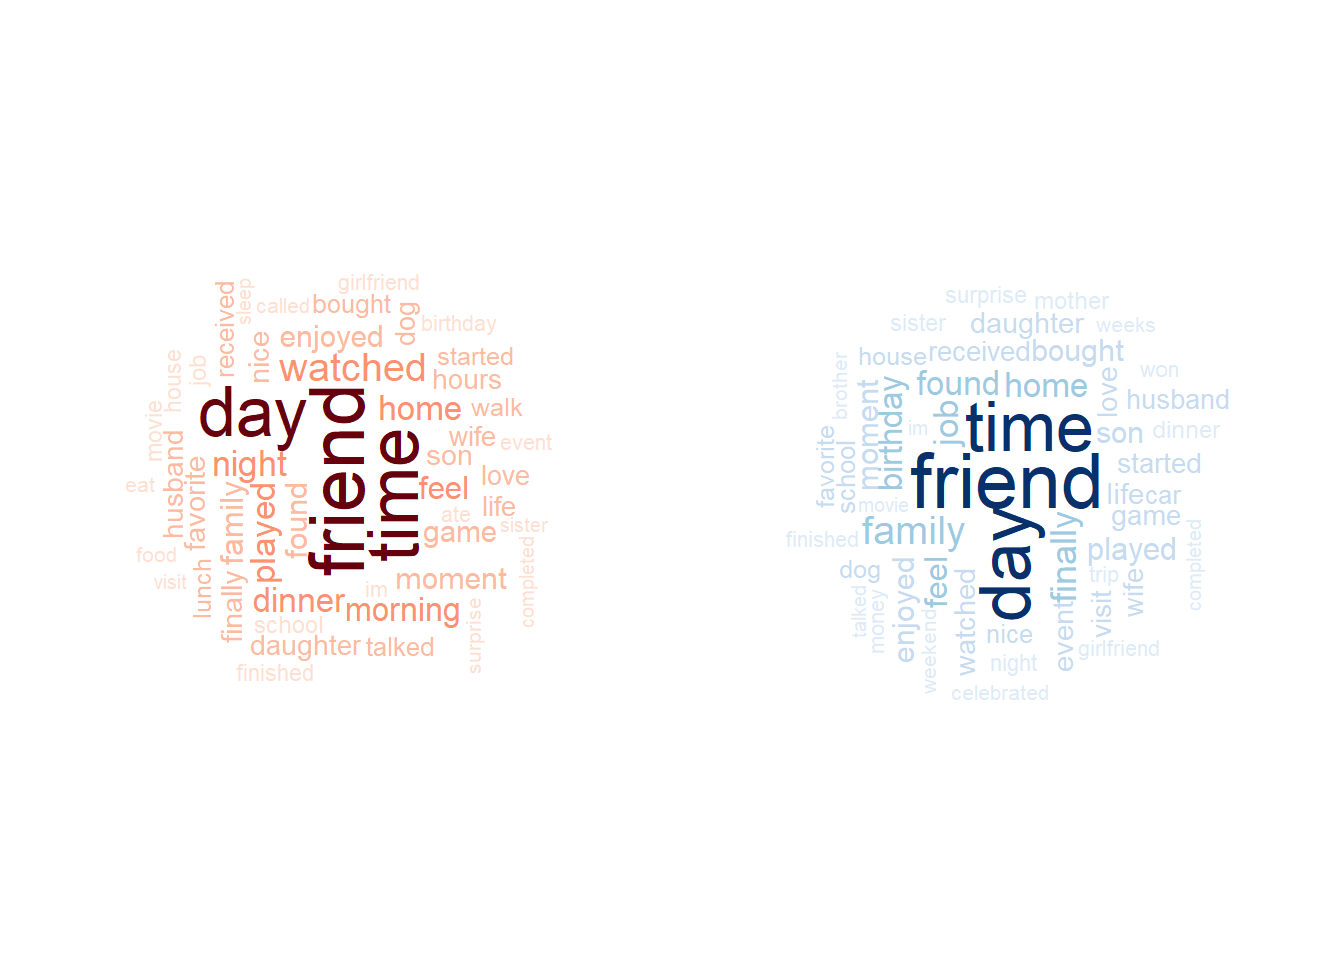
\includegraphics{preview_files/figure-latex/wordcould of single word by reflection period-1.pdf}
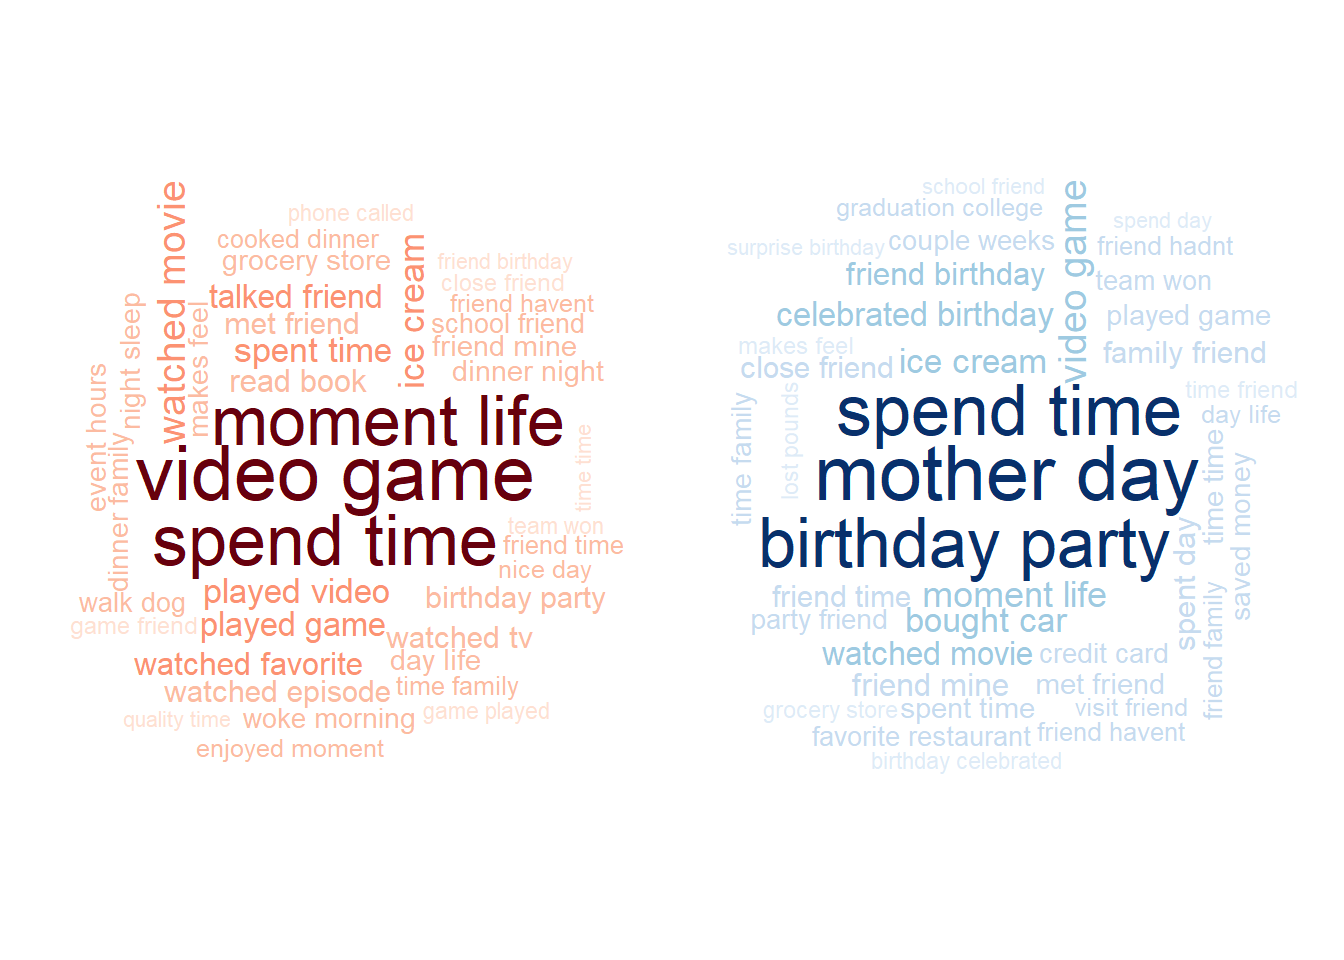
\includegraphics{preview_files/figure-latex/wordcould of pair of words by reflection period-1.pdf}
Left is the most frequent causes of happiness in 24 hours and right is
the most frequent causes of happiness in 3 months.

There are no different of the top three frequent single words. However,
``watched'', ``played'', ``night'', ``dinner'' are more frequently in 24
hours; and ``family'', ``job'', ``birthday'' are more frequently in 3
months.

In addition, ``watched movie'', ``video game'' appears more frequently
in 24 hours; and " mother day``,'' birthday party" appears more
frequently in 3 months. It seems that entertainment moments can easily
cause happiness, but do not last long. The long time happiness are
mostly because of anniversaries and festivals.

\subsubsection{Different Categories}\label{different-categories}

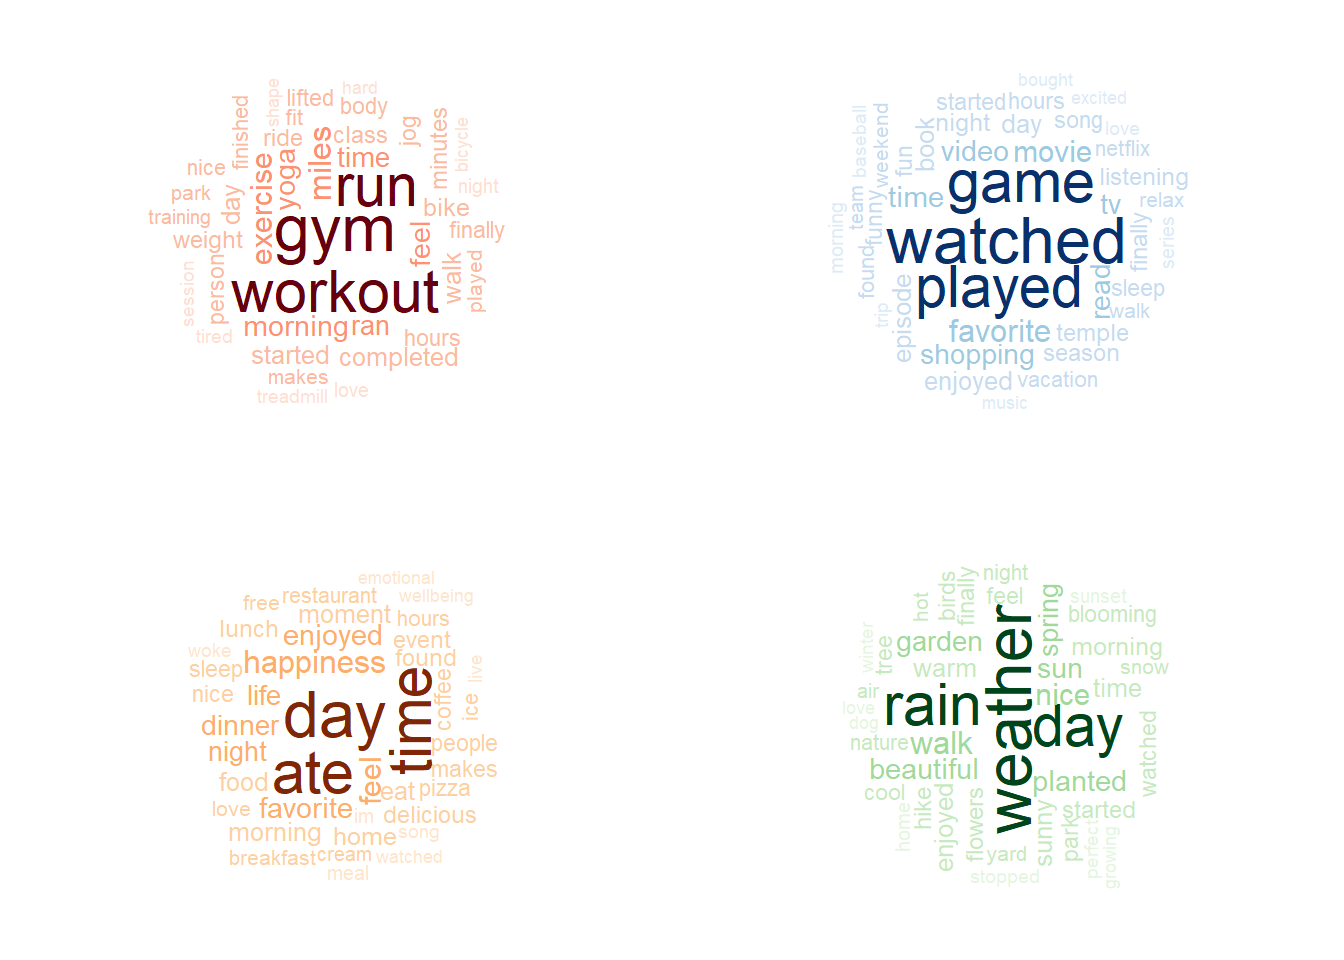
\includegraphics{preview_files/figure-latex/wordcould of single word by category-1.pdf}
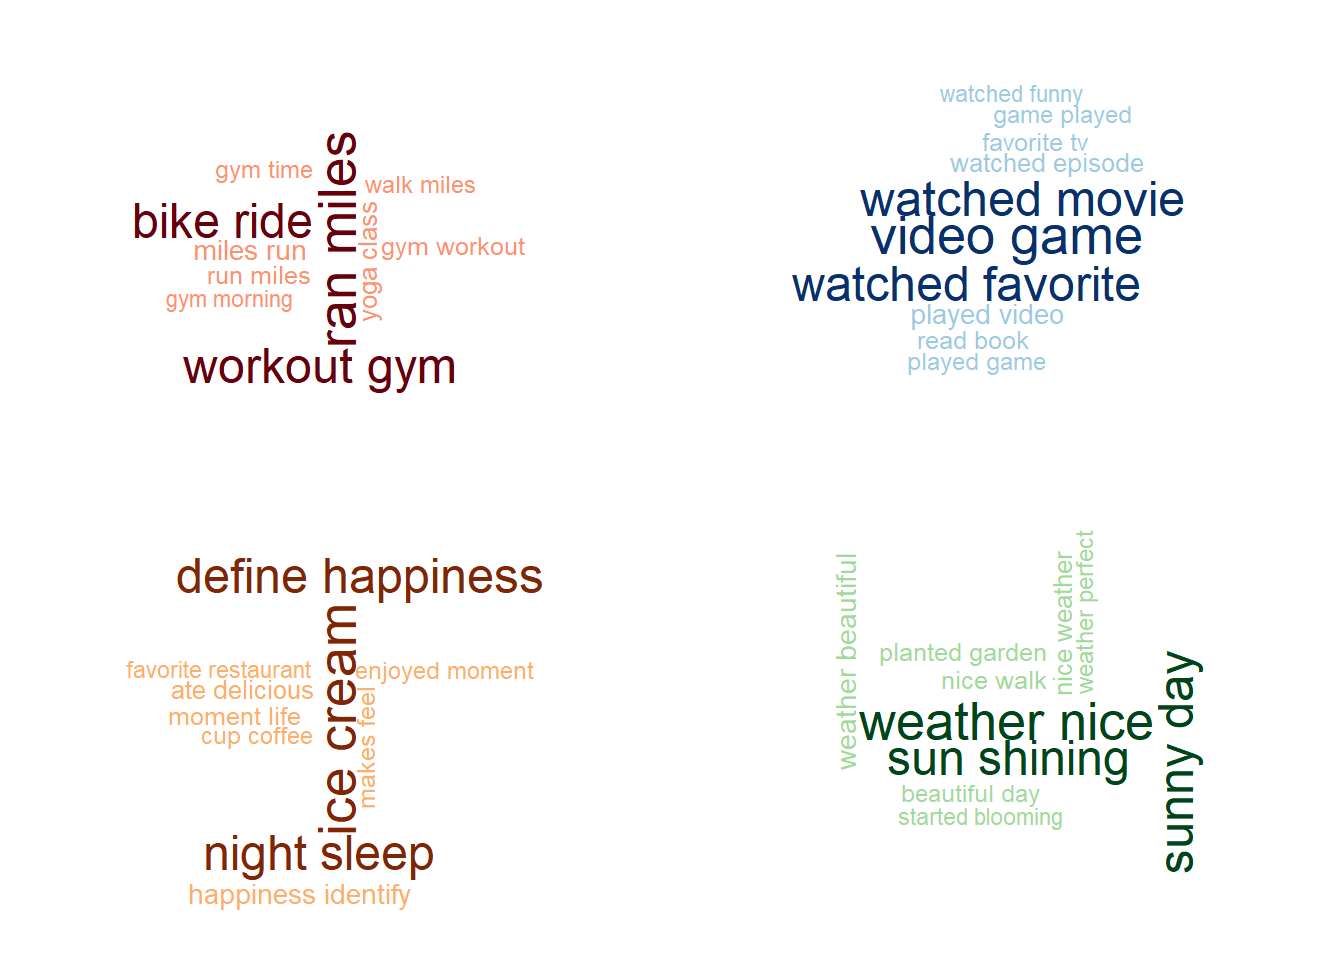
\includegraphics{preview_files/figure-latex/wordcould of pair of words by category-1.pdf}
We predicted 7 categories in previous data process. Here we randomly
chosen 4 categories for comparison.

The difference in causes of happiness are most obvious between
categories.

In single words, ``gym'', ``run'', ``workout'' are the top there
frequent causes of happiness in exercise``; watched'', ``played'',
``game'' are the top there frequent causes of happiness in leisure;
``ate'', ``day'', ``time'' are the top there frequent causes of
happiness in enjoy the moment; ``day'', ``weather'', ``rain'' are the
top there frequent causes of happiness in nature.

In pairs of words, ``workout gym'', ``ran miles'', ``bike ride'' are the
top there frequent causes of happiness in exercise; ``watched movies'',
``watched favorite'', ``video game'' are the top there frequent causes
of happiness in leisure; ``ice cream'', ``night sleep'', ``define
happiness'' are the top there frequent causes of happiness in enjoy the
moment; ``sunny day'', ``weather nice'', ``sun shining'' are the top
there frequent causes of happiness in nature.

\subsection{Topic Allocation}\label{topic-allocation}

I set the topic numbers to be 7. I manually tag them as
food\&sport``,''work
achievement``,''nature``,''feeling``,''moments``,''people\&emotion``,
and''importance day``. Because Topic''food\&sport" contains the key
words: ``coffee'', ``pizza'', ``baseball'', ``basketball'' Topic ``work
achievement'' contains ``salary'', ``promoted'', and ``paying'', Topic
``nature'' contains ``cold'', ``birds'', and ``sunset'', etc.

Based on the most popular terms and the most salient terms for each
topic, we assign a hashtag to each topic.

\subsubsection{Topic Allocation}\label{topic-allocation-1}

\includegraphics{preview_files/figure-latex/category-1.pdf} We use
heatmap to see the weight allocation of topics for predicted categories
we predicted in data processing.

Note that the red color indicates higher weights on that topic.

From the heatmap, predicted categories are most similar to the topics
allocated with higher weights. There category ``nature'' is weighted
highest with topic ``nature''; category ``leisure'' is weighted highest
with topic ``food\&sport'';category ``exercise'' is weighted highest
with topic ``nature''; category ``enjoy\_the\_moment'' is weighted
highest with topic ``moments'', topic ``bonding'' is weighted highest
with topic ``important days''; topic ``affection'' is weighted highest
with topic ``people\&emotion''; category ``achievement'' is weighted
highest with topic ``working achievement''. It is reasonable because the
corresponding category and topic describe similar terms.

\includegraphics{preview_files/figure-latex/gender-1.pdf} Now let us
look at the topic allocation among the gender.

From the heatmap, we see that the female mentions more about" people\&
emotion``,''feeling``, and''important day``; while the male mentions
more about''moments``,''natures``,''food\&sports``,and''work
achievement``. The key words match the common causes of happiness in the
two genders.

\includegraphics{preview_files/figure-latex/parethood-1.pdf} Next, let
us look at the topic allocation among parenthood.

From the heatmap, we see that the people with parenthood mention more
about ``feeling'', ``moments'', and ``people\& emotion''; while the
people without parenthood mention more about ``importance day'',
``natures'', ``food\&sports'',and ``work achievement''.

\includegraphics{preview_files/figure-latex/reflection period-1.pdf}
Finally, let us look at the topic allocation among reflection periods.

From the heatmap, we see that the people with parenthood mention more
about ``food\&sport''; while the people without parenthood mention more
about ``importance day'', ``moments'', ``people\& emotion'',
``feeling'', ``natures'' and ``work achievement''. It is reasonable the
happiness caused by food and sport usually don't last long time.

\subsection{Conclusion}\label{conclusion}

There are some general causes of happiness, like ``friends'', ``video
games'', ``spend time'', and ``moment life''. Next time if you feel
unhappy, spending time with friend or playing the video game will make
you happy most of time.

Although there are some general causes of happiness; there are some
differences in the causes of happiness between genders, parenthoods,
reflection periods, and categories.

From the Topic Modeling and Topic Allocation, we might make the
following conclusion.

\begin{itemize}
\item
  Genders: Ice cream and spending time with family can easily make women
  happy. For man, most of them will feel happy in playing video games.
  In addition, women are more easily become happy because of important
  days, like anniversary and festival. Men are more easily become happy
  because of working achievements.
\item
  Parenthood: For people with parenthood, kids and ceremonies appear in
  most of their happy moments. For people without parenthood, friend,
  food and leisure appear more frequently. In addition, people with
  parenthood are more easily to be happy because of people and their
  emotion. People without parenthood are more easily become happy
  because of working achievements, food, and sports.
\item
  reflection periods: It seems that entertainment moments can easily
  cause happiness, but do not last long. The long-time happiness is
  mostly because of anniversaries and festivals.
\item
  Category: The difference in causes of happiness are most obvious
  between categories. Predicted categories are the most like the topics
  allocated with higher weights. There are different ways and different
  categories to be happy. If we chose the most frequently causes of
  happiness followed our gender, parenthood, reflection period and
  favorite category, we might can be happy more easily.
\end{itemize}


\end{document}
